\documentclass[handout,8pt]{beamer}
\usepackage[UKenglish]{babel}
\usepackage[UKenglish]{isodate}
\usepackage{graphicx}
\usepackage{tikz}
\usepackage{bm}
\usepackage{bbm}
\usepackage{mathtools}
\usepackage{pgfpages}

\pgfpagesuselayout{2 on 1}[a4paper]
\pgfpageslogicalpageoptions{1}{center = \pgfpoint{.5\pgfphysicalwidth}{.72\pgfphysicalheight}}
\pgfpageslogicalpageoptions{2}{center = \pgfpoint{.5\pgfphysicalwidth}{.28\pgfphysicalheight}}

\beamertemplatenavigationsymbolsempty
\usetikzlibrary{shapes,bayesnet}
\newtheorem{proposition}{Proposition}
\DeclareMathOperator*{\argmax}{arg\,max}
\DeclareMathOperator{\diag}{diag}
\DeclareMathOperator{\tr}{tr}
\newcommand{\Kuu}{\mathbf{K}_{\mathbf{u},\mathbf{u}}}
\newcommand{\Krr}{\mathbf{K}_{\mathbf{r},\mathbf{r}}}
\newcommand{\Kru}{\mathbf{K}_{\mathbf{r},\mathbf{u}}}
\newcommand{\rinf}{\lVert \mathbf{r} \rVert_\infty}
\newcommand{\vbound}{\frac{\rinf + \log|\mathcal{A}|}{1 - \gamma}}
\newcommand{\dt}{\frac{\partial}{\partial t}}
\newcommand{\dx}{\,d\mathbf{r}\,d\mathbf{u}}

\DeclarePairedDelimiterX{\infdivx}[2]{(}{)}{%
  #1\;\delimsize\|\;#2%
}
\newcommand{\DKL}{D_{\mathrm{KL}}\infdivx}

\author{Paulius Dilkas}
\title{Variational Inference for Inverse Reinforcement Learning with Gaussian
  Processes}
\date{15th January 2019}

\begin{document}

\begin{frame}{Markov Decision Process}
  \begin{minipage}[t][0.85\textheight]{\textwidth}
    $\mathcal{M} = (\mathcal{S}, \mathcal{A}, \mathcal{T}, \gamma, \mathbf{r})$,
    where
  
    $\mathcal{T} : \mathcal{S} \times \mathcal{A} \times \mathcal{S} \to [0,
    1]$, and

    $\mathbf{r} \in \mathbb{R}^{|\mathcal{S}|} \text{ or } r : \mathcal{S} \to
    \mathbb{R}$.
    \begin{tikzpicture}[state/.style={rectangle, draw, scale=1.5},
      action/.style={diamond, draw, fill=lightgray}, overlay, shift={(-2, -3)}]
      \node(origin) at (0, 0){};
      \node[state](s0) at (1, 0){$s_0$};
      \node[action](start) at (2.5, 0){start};
      \node[state,label=try](s1) at (4, 0){$s_1$};
      \node[action](wait) at (4, -2){wait};
      \node[action](send) at (5.5, 0){send};
      \node[state,label={right:failure},label={below:\textcolor{red}{-1}}](s2) at (7, 2){$s_2$};
      \node[action](restart) at (7, 4){restart};
      \node[state,label={left:success},label={above:\textcolor{green}{+3}}](s3) at (7, -2){$s_3$};
      \node[action](stop) at (8.5, -2){stop};
      \draw[->] (s0) edge (start);
      \draw[->] (start) edge node[above] {$1$} (s1);
      \draw[->,bend left] (s1) edge (wait);
      \draw[->,bend left] (wait) edge node[left] {$1$} (s1);
      \draw[->] (s1) edge (send);
      \draw[->] (send) edge node[left] {$0.01$} (s2);
      \draw[->] (send) edge node[left] {$0.99$} (s3);
      \draw[->] (s2) edge (restart);
      \draw[->,bend right] (restart) edge node[above] {$1$} (s0);
      \draw[->,bend left] (s3) edge (stop);
      \draw[->,bend left] (stop) edge node[below] {$1$} (s3);
      \draw[->] (origin) edge (s0);
    \end{tikzpicture}
  \end{minipage}
\end{frame}

\begin{frame}{Inverse Reinforcement Learning}
  Given:
  \begin{itemize}
  \item $\mathcal{M} \setminus \{ \mathbf{r} \}$,
  \item $\mathcal{D} = \{ \zeta_i \}_{i=1}^N$, where $\zeta_i = \{ (s_{i,1},
    a_{i,1}), \dots, (s_{i,T}, a_{i,T}) \}$,
  \item features $\mathbf{X} \in \mathbb{R}^{|\mathcal{S}| \times d}$,
  \end{itemize}
  find $\mathbf{r}$. Motivation:
  \begin{itemize}
  \item Reward functions can be difficult to construct in practice
  \item Rewards are more generalisable than policies
  \end{itemize}
  \begin{block}{Applications}
    \begin{columns}[T]
      \begin{column}{0.5\textwidth}
        \begin{itemize}
        \item Autonomous vehicle control
          \begin{itemize}
          \item Helicopter tricks
          \item Robot movement among people
          \end{itemize}
        \item Predicting behaviour
          \begin{itemize}
          \item Taxi destinations
          \item Pedestrian movement
          \item Energy efficient driving
          \end{itemize}
        \end{itemize}
      \end{column}
      \begin{column}{0.5\textwidth}
        \begin{figure}
          \centering
          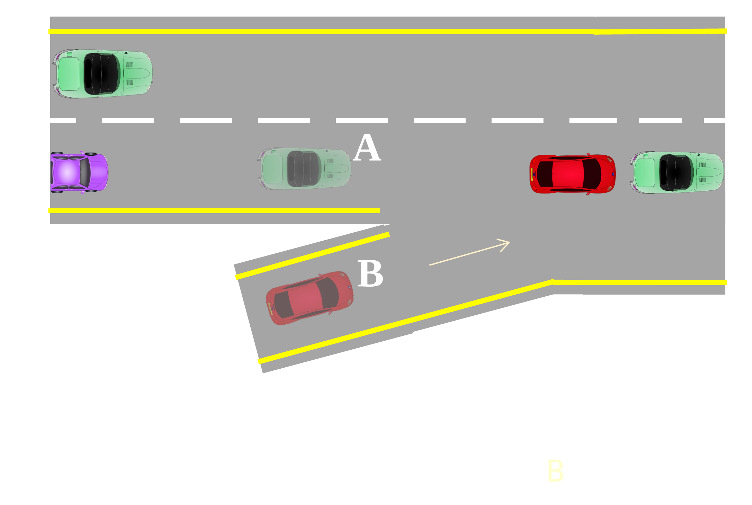
\includegraphics[width=\textwidth]{cars.png}
        \end{figure}
      \end{column}
    \end{columns}
  \end{block}
\end{frame}

\begin{frame}{Variational Inference}
  How to calculate the posterior probability distribution?
  \[
    p(\mathbf{r}, \mathbf{u} \mid \mathcal{D}) = \frac{p(\mathcal{D} \mid
      \mathbf{r})p(\mathbf{r} \mid \mathbf{u})p(\mathbf{u})}{p(\mathcal{D})}
  \]
  Solution: approximate $p(\mathbf{r}, \mathbf{u} \mid \mathcal{D})$ with
  $q(\mathbf{r}, \mathbf{u}) = q(\mathbf{r} \mid \mathbf{u})q(\mathbf{u})$, where
  \begin{columns}[onlytextwidth,T]
    \begin{column}{0.4\textwidth}
      \begin{itemize}
      \item $q(\mathbf{r} \mid \mathbf{u}) = p(\mathbf{r} \mid \mathbf{u})$,
      \item $q(\mathbf{u}) = \mathcal{N}(\mathbf{u}; \bm\mu, \bm\Sigma)$.
      \end{itemize}
    \end{column}
    \begin{column}{0.6\textwidth}
      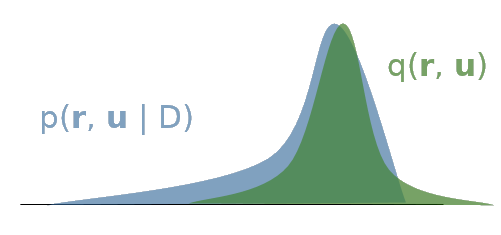
\includegraphics[scale=1]{vi.png}
    \end{column}
  \end{columns}
  \begin{block}{Benefits}
    \begin{itemize}
    \item More precise reward predictions
    \item Variance estimates guide further data collection
    \item Bayesian treatment guards against overfitting
    \end{itemize}
  \end{block}
\end{frame}

\begin{frame}{Theoretical Results}
  \begin{proposition}
    MDP value functions $V(s) : \mathbb{R}^{|\mathcal{S}|} \to \mathbb{R}$ (for
    $s \in \mathcal{S}$) are Lebesgue measurable.
  \end{proposition}
  \begin{proposition}
    If the initial values of the MDP value function satisfy the following
    bound, then the bound remains satisfied throughout value iteration:
    \[
      |V_{\mathbf{r}}(s)| \le \vbound.
    \]
  \end{proposition}
  \begin{theorem} \label{thm:main}
    Whenever the derivative exists,
    \[
      \dt\iint
      V_{\mathbf{r}}(s)q(\mathbf{r} \mid \mathbf{u})q(\mathbf{u})\dx
      = \iint
      \dt[V_{\mathbf{r}}(s)q(\mathbf{r} \mid \mathbf{u})q(\mathbf{u})]\dx,
    \]
    where $t$ is any scalar part of $\bm\mu$, $\bm\Sigma$, or $\bm\lambda$.
  \end{theorem}
\end{frame}
\end{document}